% !TEX program = xelatex
\documentclass[UTF8]{ctexart}
% \usepackage{xeCJK}
\usepackage{amsmath}
\usepackage{amssymb}
\usepackage{geometry}
\geometry{a4paper,scale=0.8}
\usepackage{multicol}
\author{2017211123 褚逸豪}
\title{1234的可能合法出栈序列}
\begin{document}
\maketitle
\section{多少种解?}
显然,通过组合数学相关知识,我们知道答案是$C_4$,即
$$\frac{1}{5}\binom 8 4=14$$
我们亦可通过递推的方式进行解算:
\begin{center}
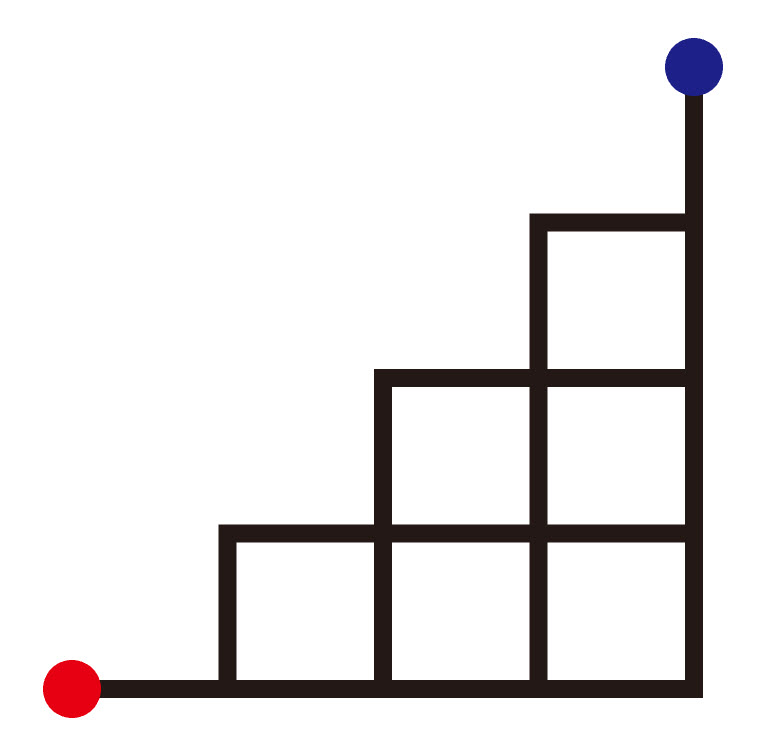
\includegraphics[scale=0.5]{sample.jpg}
\end{center}
将向右移动看作入栈,向上移动看作出栈,则答案应为从红点到蓝点的有效路径条数\\
易得递推式:
$$f_{x,y} = f_{x-1,y}[x>y]+f_{x,y-1}[y \geqslant 1]$$
初始条件
$$f_{1,1}=1$$
\section{解都有哪些?}
我们可以根据以上的那张图求出全部的合法出栈序列,例如路径(1,1)->(1,2)->(1,3)->(1,4)->(2,4)->(3,4)->(4,4)对应的出栈序列是“4 3 2 1”\\
所有出栈序列如下
\begin{multicols}{2}\begin{center}\noindent
4 3 2 1\\
3 4 2 1\\
3 2 4 1\\
3 2 1 4\\
2 4 3 1\\
2 3 4 1\\
2 3 1 4\\
2 1 4 3\\
2 1 3 4\\
1 4 3 2\\
1 3 4 2\\
1 3 2 4\\
1 2 4 3\\
1 2 3 4\end{center}
\end{multicols}
\end{document}